\documentclass[12pt]{article}\usepackage[]{graphicx}\usepackage[]{color}
%% maxwidth is the original width if it is less than linewidth
%% otherwise use linewidth (to make sure the graphics do not exceed the margin)
\makeatletter
\def\maxwidth{ %
  \ifdim\Gin@nat@width>\linewidth
    \linewidth
  \else
    \Gin@nat@width
  \fi
}
\makeatother

\definecolor{fgcolor}{rgb}{0.345, 0.345, 0.345}
\newcommand{\hlnum}[1]{\textcolor[rgb]{0.686,0.059,0.569}{#1}}%
\newcommand{\hlstr}[1]{\textcolor[rgb]{0.192,0.494,0.8}{#1}}%
\newcommand{\hlcom}[1]{\textcolor[rgb]{0.678,0.584,0.686}{\textit{#1}}}%
\newcommand{\hlopt}[1]{\textcolor[rgb]{0,0,0}{#1}}%
\newcommand{\hlstd}[1]{\textcolor[rgb]{0.345,0.345,0.345}{#1}}%
\newcommand{\hlkwa}[1]{\textcolor[rgb]{0.161,0.373,0.58}{\textbf{#1}}}%
\newcommand{\hlkwb}[1]{\textcolor[rgb]{0.69,0.353,0.396}{#1}}%
\newcommand{\hlkwc}[1]{\textcolor[rgb]{0.333,0.667,0.333}{#1}}%
\newcommand{\hlkwd}[1]{\textcolor[rgb]{0.737,0.353,0.396}{\textbf{#1}}}%
\let\hlipl\hlkwb

\usepackage{framed}
\makeatletter
\newenvironment{kframe}{%
 \def\at@end@of@kframe{}%
 \ifinner\ifhmode%
  \def\at@end@of@kframe{\end{minipage}}%
  \begin{minipage}{\columnwidth}%
 \fi\fi%
 \def\FrameCommand##1{\hskip\@totalleftmargin \hskip-\fboxsep
 \colorbox{shadecolor}{##1}\hskip-\fboxsep
     % There is no \\@totalrightmargin, so:
     \hskip-\linewidth \hskip-\@totalleftmargin \hskip\columnwidth}%
 \MakeFramed {\advance\hsize-\width
   \@totalleftmargin\z@ \linewidth\hsize
   \@setminipage}}%
 {\par\unskip\endMakeFramed%
 \at@end@of@kframe}
\makeatother

\definecolor{shadecolor}{rgb}{.97, .97, .97}
\definecolor{messagecolor}{rgb}{0, 0, 0}
\definecolor{warningcolor}{rgb}{1, 0, 1}
\definecolor{errorcolor}{rgb}{1, 0, 0}
\newenvironment{knitrout}{}{} % an empty environment to be redefined in TeX

\usepackage{alltt}
 
\usepackage[margin=1in]{geometry}
\usepackage{amsmath,amsthm,amssymb, mathtools}
\usepackage[T1]{fontenc}
\usepackage{lmodern}
\usepackage{fixltx2e}
\usepackage[shortlabels]{enumitem}
\usepackage{mathrsfs}
 
\newcommand{\N}{\mathbb{N}}
\newcommand{\R}{\mathbb{R}}
\newcommand{\Z}{\mathbb{Z}}
\newcommand{\Q}{\mathbb{Q}}
 
\newenvironment{theorem}[2][Theorem]{\begin{trivlist}
\item[\hskip \labelsep {\bfseries #1}\hskip \labelsep {\bfseries #2.}]}{\end{trivlist}}
\newenvironment{lemma}[2][Lemma]{\begin{trivlist}
\item[\hskip \labelsep {\bfseries #1}\hskip \labelsep {\bfseries #2.}]}{\end{trivlist}}
\newenvironment{exercise}[2][Exercise]{\begin{trivlist}
\item[\hskip \labelsep {\bfseries #1}\hskip \labelsep {\bfseries #2.}]}{\end{trivlist}}
\newenvironment{problem}[2][Problem]{\begin{trivlist}
\item[\hskip \labelsep {\bfseries #1}\hskip \labelsep {\bfseries #2.}]}{\end{trivlist}}
\newenvironment{question}[2][Question]{\begin{trivlist}
\item[\hskip \labelsep {\bfseries #1}\hskip \labelsep {\bfseries #2.}]}{\end{trivlist}}
\newenvironment{corollary}[2][Corollary]{\begin{trivlist}
\item[\hskip \labelsep {\bfseries #1}\hskip \labelsep {\bfseries #2.}]}{\end{trivlist}}
\newcommand{\textfrac}[2]{\dfrac{\text{#1}}{\text{#2}}}

\DeclareMathOperator{\proj}{proj}
\newcommand{\vct}{\mathbf}
\newcommand{\vctproj}[2][]{\proj_{\vct{#1}}\vct{#2}}
\IfFileExists{upquote.sty}{\usepackage{upquote}}{}
\begin{document}

\title{Advanced Mathematical Statistics: Assignment 2}

\author{Chris Hayduk}
\date{October 3, 2019}

\maketitle




\begin{problem}{4.2}
\end{problem}

\begin{enumerate}[a)]

\item $f(x_1, x_2) = \frac{1}{2\pi\sqrt{1.5}} \times \exp\{-\frac{2}{3}[\left(\frac{x_1}{\sqrt{2}}\right)^2 + \left(x_2 - 2\right)^2 - \left(\frac{x_1}{\sqrt{2}}\right)\left(x_2 - 2\right)]\}$

\item We have that $\rho_{12} = 0.5 \implies \sigma_{12} = 0.5(\sqrt{\sigma_{11}\sigma_{22}}) = 0.5(\sqrt{2})$. So,
\begin{align*}
&(\vct{x} - \vct{\mu})'\Sigma^{-1}(\vct{x} - \vct{\mu})\\
&= \begin{bmatrix} x_1 - \mu_1 & x_2 - \mu_2 \end{bmatrix} \frac{1}{\sigma_{11}\sigma_{22}-\sigma_{12}^2} \begin{bmatrix} \sigma_{22} & -\sigma_{12} \\ -\sigma_{12} & \sigma_{11} \end{bmatrix} \begin{bmatrix} x_1 - \mu_1 \\ x_2 - \mu_2 \end{bmatrix}\\
&= \begin{bmatrix} x_1 & x_2 - 2 \end{bmatrix} \frac{1}{2-(0.5\sqrt{2})^2} \begin{bmatrix} 1 & -0.5\sqrt{2} \\ -0.5\sqrt{2} & 2 \end{bmatrix} \begin{bmatrix} x_1 \\ x_2 - 2 \end{bmatrix}\\
&= \begin{bmatrix} \frac{2}{3} x_1 + (\frac{-\sqrt{2}}{3})(x_2 - 2) & (\frac{-\sqrt{2}}{3})(x_1 ) + \frac{4}{3}(x_2 - 2) \end{bmatrix} \begin{bmatrix} x_1 \\ x_2 - 2 \end{bmatrix}\\
&= x_1\left(\frac{2}{3} x_1 + \left(\frac{-\sqrt{2}}{3}\right)(x_2 - 2)\right) + (x_2 - 2)\left(\left(\frac{-\sqrt{2}}{3}\right)x_1 + \frac{4}{3}(x_2 - 2)\right)\\
&= \frac{2}{3}x_1^2 + \left(\frac{-\sqrt{2}}{3}\right)(x_2 - 2)x_1 + (x_2 - 2)\left(\frac{-\sqrt{2}}{3}\right)x_1 + \frac{4}{3}(x_2 - 2)^2\\
&= \frac{2}{3}x_1^2 + \frac{-2\sqrt{2}(x_2x_1 - 2x_1)}{3} + \frac{4}{3}x_2^2 - \frac{16}{3}x_2 + \frac{16}{3}
\end{align*}

\item $c^2 = \chi^2_2(0.5) \approx 1.386294$. So we take 
\begin{align*}
\frac{2}{3}x_1^2 + \frac{-2\sqrt{2}(x_2x_1 - 2x_1)}{3} + \frac{4}{3}x_2^2 - \frac{16}{3}x_2 + \frac{16}{3} = 1.386294
\end{align*}
to be the surface of the ellipsoid containing 50\% of the probability. The graph for this can be seen below.

\begin{knitrout}
\definecolor{shadecolor}{rgb}{0.969, 0.969, 0.969}\color{fgcolor}
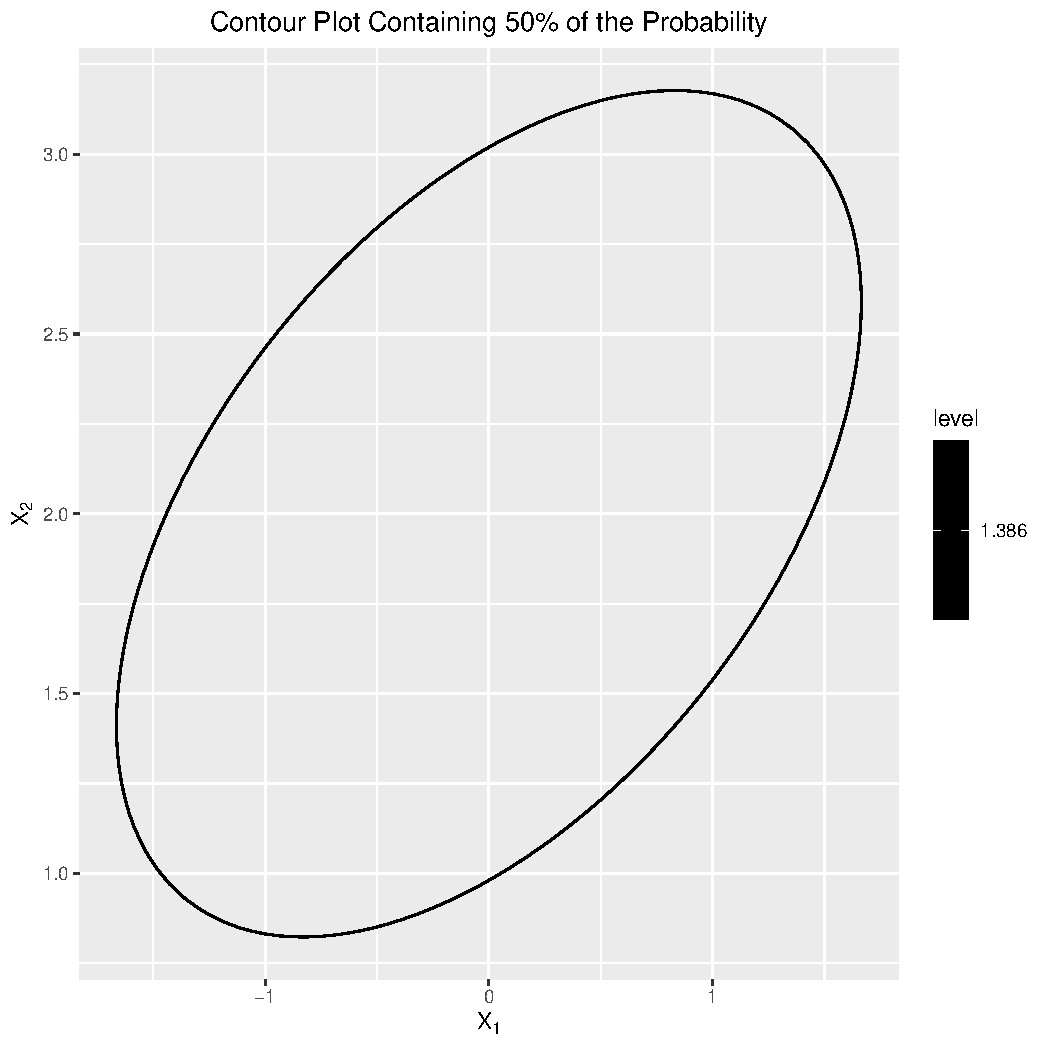
\includegraphics[width=\maxwidth]{figure/unnamed-chunk-2-1} 

\end{knitrout}
\end{enumerate}

%%%%%%%%%%%%%%%%%%%%%%%%%%%%%%%%%%%%%%%%%%%%%%%%%%%%%%%%%%%%%%%%%%%%%%%%%%%%%%%%%%%%%%%%%%%%%%%%%%%%%%%%%%%%%%%%%%%%%%%%%%%%%%%%%%%%%

\begin{problem}{4.3}
\end{problem}

\begin{enumerate}[a)]

\item $X_1$ and $X_2$ are not independent because $\sigma_{12} = \sigma_{21} = -2 \neq 0$.

\item $X_2$ and $X_3$ are independent because $\sigma_{23} = \sigma_{32} = 0$.

\item If we partition the covariance matrix into $(X_1, X_2)$ and $X_3$ partitions, we get
\begin{align*}
\left[\begin{array}{@{}cc|c@{}}
    1 & -2 & 0 \\
    -2 & 5 & 0 \\\hline
    0 & 0 & 2
  \end{array}\right]
\end{align*}

Thus, we can see that the two diagonal sections of the matrix have the forms $\vct{0}, \vct{0}'$. As a result, $(X_1, X_2)$ and $X_3$ are independent.

\item Let $\vct{A} = \begin{bmatrix} \frac{1}{2} & \frac{1}{2} & 0 \\ 0 & 0 & 1\end{bmatrix}$. From Result 4.3, we know $\vct{A}\vct{X}$ is distributed as $N_q(\vct{A}\vct{\mu}, \vct{A}\vct{\Sigma}\vct{A}')$ with $q = 2$ in this case.

So we have,
\begin{align*}
\vct{A}\vct{\Sigma}\vct{A}' &= \begin{bmatrix} \frac{1}{2} & \frac{1}{2} & 0 \\ 0 & 0 & 1\end{bmatrix} \begin{bmatrix} 1 & -2 & 0 \\ -2 & 5 & 0 \\ 0 & 0 & 2 \end{bmatrix} \begin{bmatrix} \frac{1}{2} & 0 \\ \frac{1}{2} & 0 \\ 0 & 1\end{bmatrix}\\
&= \begin{bmatrix} -\frac{1}{2} & \frac{3}{2} & 0 \\ 0 & 0 & 2\end{bmatrix} \begin{bmatrix} \frac{1}{2} & 0 \\ \frac{1}{2} & 0 \\ 0 & 1\end{bmatrix}\\
&= \begin{bmatrix} \frac{1}{2} & 0 \\ 0 & 2 \end{bmatrix}
\end{align*}

As can be clearly seen from the above matrix, $\vct{A}\vct{\Sigma}\vct{A}'$, the covariance between $\frac{X_1 + X_2}{2}$ and $X_3$ is 0. As a result, $\frac{X_1 + X_2}{2}$ and $X_3$ are independent.

\item Let $\vct{A} = \begin{bmatrix} 0 & 1 & 0 \\ -\frac{5}{2} & 1 & -1\end{bmatrix}$. From Result 4.3, we know $\vct{A}\vct{X}$ is distributed as $N_q(\vct{A}\vct{\mu}, \vct{A}\vct{\Sigma}\vct{A}')$ with $q = 2$ in this case.

So we have,
\begin{align*}
\vct{A}\vct{\Sigma}\vct{A}' &= \begin{bmatrix} 0 & 1 & 0 \\ -\frac{5}{2} & 1 & -1\end{bmatrix} \begin{bmatrix} 1 & -2 & 0 \\ -2 & 5 & 0 \\ 0 & 0 & 2 \end{bmatrix} \begin{bmatrix} 0 & -\frac{5}{2} \\ 1 & 1 \\ 0 & -1\end{bmatrix}\\
&= \begin{bmatrix} -2 & 5 & 0 \\ -\frac{9}{2} & 10 & -2\end{bmatrix} \begin{bmatrix} 0 & -\frac{5}{2} \\ 1 & 1 \\ 0 & -1\end{bmatrix}\\
&= \begin{bmatrix} 5 & 10 \\ 10 & \frac{93}{4} \end{bmatrix}
\end{align*}

We can see from the above matrix that the covariance between the random variables is not 0. Thus, $X_2$ and $X_2 - \frac{5}{2}X_1 - X_3$ are not independent.
\end{enumerate}

%%%%%%%%%%%%%%%%%%%%%%%%%%%%%%%%%%%%%%%%%%%%%%%%%%%%%%%%%%%%%%%%%%%%%%%%%%%%%%%%%%%%%%%%%%%%%%%%%%%%%%%%%%%%%%%%%%%%%%%%%%%%%%%%%%%%%

\begin{problem}{4.4}
\end{problem}

\begin{enumerate}[a)]

\item Let $A = \begin{bmatrix} 3 & -2 & 1 \end{bmatrix}$. By Result 4.3, $3X_1 - 2X_2 + X_3$ is distributed as $N_1(\vct{A}\vct{\mu}, \vct{A}\vct{\Sigma}\vct{A}')$ with mean vector and covariance matrix,
\begin{align*}
&\vct{A}\vct{\mu} = 6 + 6 + 1 = 13\\
&\vct{A}\vct{\Sigma}\vct{A}' = \begin{bmatrix} 2 & -1 & 1 \end{bmatrix}\vct{A}' = 6 + 2 + 1 = 9
\end{align*}

\item Let $A = \begin{bmatrix} 0 & 1 & 0 \\ -a_1 & 1 & -a_2 \end{bmatrix}$.\\

Now find $\vct{A}\vct{\Sigma}\vct{A}'$:
\begin{align*}
\vct{A}\vct{\Sigma}\vct{A}' &= \begin{bmatrix} 1 & 3 & 2 \\ -a_1 + 1 - a_2 & -a_1 + 3 - 2a_2 & a_1 + 2 - 2a_2 \end{bmatrix}\begin{bmatrix} 0 & -a_1 \\ 1 & 1 \\ 0 & -a_2 \end{bmatrix}\\
&= \begin{bmatrix} 3 & -a_1 + 3 - 2a_2 \\ -a_1 + 3 - 2a_2 & (-a_1)^2 - 2a_1 - 2a_1a_2 + 3 - 4a_2 + 2(-a_2)^2  \end{bmatrix}
\end{align*}

In order for the covariance to be 0 (ie. $X_2$ and $-a_1X_1 + X_2 - a_3X_3$ independent), we need $-a_1 + 3 - 2a_2 = 0$. That is, $a_1 + 2a_2 = 3$. For instance, take $a_1 = 1$ and $a_2 = 1$. Then we have,
\begin{align*}
\vct{A}\vct{\Sigma}\vct{A}' = \begin{bmatrix} 3 & 0 \\ 0 & -2 \end{bmatrix}
\end{align*}
\end{enumerate}

Thus, if $\vct{a} = \begin{bmatrix} a_1 \\ a_2 \end{bmatrix} = \begin{bmatrix} 1 \\ 1 \end{bmatrix}$, then we have that $X_2$ and $X_2 - \vct{a}'\begin{bmatrix} X_1 \\ X_3 \end{bmatrix}$ are independent.

%%%%%%%%%%%%%%%%%%%%%%%%%%%%%%%%%%%%%%%%%%%%%%%%%%%%%%%%%%%%%%%%%%%%%%%%%%%%%%%%%%%%%%%%%%%%%%%%%%%%%%%%%%%%%%%%%%%%%%%%%%%%%%%%%%%%%

\begin{problem}{4.5}
\end{problem}

\begin{enumerate}[a)]

\item By Result 4.6, we have 
\begin{align*}
\mu &= \mu_1 + \sigma_{12}(\sigma_{22})^{-1}(x_2 - \mu_2)\\
&= 0 + 0.5(\sqrt{2})(1)^{-1}(x_2 - 2)\\
&= 0.5(\sqrt{2})x_2 - \sqrt{2}
\end{align*}

In addition, we have 
\begin{align*}
\sigma &= \sigma_{11} - \sigma_{12}(\sigma_{22})^{-1}\sigma_{21}\\
&= 2 - 0.5(\sqrt{2})(1)^{-1}0.5(\sqrt{2})\\
&= 2 - 0.25(2) = 1.5
\end{align*}

\item Let's rearrange the $\vct{\Sigma}$ matrix,
\begin{align*}
\vct{\Sigma} &= \begin{bmatrix} 1 & 0 & -2 \\
                    0 & 2 & 0 \\
                    -2 & 0 & 5
    \end{bmatrix}\\
&= \left[\begin{array}{@{}cc|c@{}}
    1 & 0 & -2 \\
    0 & 2 & 0 \\\hline
    -2 & 0 & 5
  \end{array}\right]
\end{align*}\\

and the $\vct{\mu}$ vector,
\begin{align*}
\vct{\mu} &= \begin{bmatrix} -3 \\ 4 \\ 1 \end{bmatrix}\\
&= \left[\begin{array}{@{}c@{}}
    -3 \\
    4 \\\hline
    1
  \end{array}\right]
\end{align*}

Then we have,
\begin{align*}
\vct{\mu} &= \vct{\mu}_1 + \vct{\Sigma}_{12}\vct{\Sigma}_{22}^{-1}(x_2 - \vct{\mu}_2)\\
&= \begin{bmatrix} -3 \\ 4 \end{bmatrix} + \begin{bmatrix} -2 \\ 0 \end{bmatrix} (\frac{1}{5})(x_2 - 1)\\
&= \begin{bmatrix} -3 \\ 4 \end{bmatrix} + \begin{bmatrix} -2 \\ 0 \end{bmatrix} (\frac{1}{5}x_2 - \frac{1}{5})
\end{align*}

and,
\begin{align*}
\vct{\Sigma} &= \Sigma_{11} - \Sigma_{12}\Sigma_{22}^{-1}\Sigma_{21}\\
&= \begin{bmatrix} 1 & 0 \\ 0 & 2 \end{bmatrix} - \begin{bmatrix} -2 \\ 0 \end{bmatrix} \left(\frac{1}{5}\right) \begin{bmatrix} -2 & 0 \end{bmatrix}\\
&= \begin{bmatrix} 1 & 0 \\ 0 & 2 \end{bmatrix} - \begin{bmatrix} -2 \\ 0 \end{bmatrix} \begin{bmatrix} -\frac{2}{5} & 0 \end{bmatrix}\\
&= \begin{bmatrix} 1 & 0 \\ 0 & 2 \end{bmatrix} - \begin{bmatrix} \frac{4}{5} & 0 \\ 0 & 0 \end{bmatrix}\\
&= \begin{bmatrix} \frac{1}{5} & 0 \\ 0 & 2 \end{bmatrix}
\end{align*}


\item If we partition the covariance matrix into $(X_1, X_2)$ and $X_3$ partitions, we get
\begin{align*}
\vct{\Sigma} &= \left[\begin{array}{@{}cc|c@{}}
    1 & 1 & 1 \\
    1 & 3 & 2 \\\hline
    1 & 2 & 2
  \end{array}\right]\\
&=\left[\begin{array}{@{}c|c@{}}
    \vct{\Sigma}_{11} & \vct{\Sigma}_{12} \\\hline
    \vct{\Sigma}_{21} & \vct{\Sigma}_{22}
  \end{array}\right]
\end{align*}

and,
\begin{align*}
\vct{\mu} &= \left[\begin{array}{@{}c@{}}
    2 \\
    -3 \\\hline
    1
  \end{array}\right]\\
&= \left[\begin{array}{@{}c@{}}
    \vct{\mu}_1 \\\hline
    \vct{\mu}_2
  \end{array}\right]
\end{align*}


So we have,
\begin{align*}
\mu &= \vct{\mu}_2 + \vct{\Sigma}_{21}(\vct{\Sigma}_{11})^{-1}(x_1 - \vct{\mu}_1)\\
&= 1 + \begin{bmatrix} 1 & 2 \end{bmatrix}\left(\begin{bmatrix} \frac{3}{2} & -\frac{1}{2} \\ -\frac{1}{2} & \frac{1}{2} \end{bmatrix}\right)(x_1 - \begin{bmatrix} 2 \\ -3 \end{bmatrix})\\
&= 1 + \left(\begin{bmatrix} \frac{1}{2} & \frac{1}{2} \end{bmatrix}\right)(x_1 - \begin{bmatrix} 2 \\ -3 \end{bmatrix})\\
&= 1 + \left(\begin{bmatrix} \frac{1}{2} & \frac{1}{2} \end{bmatrix}\right)\left(\begin{bmatrix} X_1 \\ X_2 \end{bmatrix} - \begin{bmatrix} 2 \\ -3 \end{bmatrix}\right)\\
&= 1 + \left(\begin{bmatrix} \frac{1}{2} & \frac{1}{2} \end{bmatrix}\right)\left(\begin{bmatrix} X_1 - 2 \\ X_2 + 3 \end{bmatrix}\right)\\
&= 1 + \frac{1}{2}\left(X_1 - 2 + X_2 + 3\right)\\
&= \frac{1}{2}X_1 + \frac{1}{2}X_2 + \frac{3}{2}
\end{align*}

and,
\begin{align*}
\vct{\Sigma} &= \vct{\Sigma}_{22} - \vct{\Sigma}_{21}\left(\vct{\Sigma}_{11}\right)^{-1}\vct{\Sigma}_{12}\\
&= 2 - \begin{bmatrix} 1 & 2 \end{bmatrix}\left(\begin{bmatrix} \frac{3}{2} & -\frac{1}{2} \\ -\frac{1}{2} & \frac{1}{2} \end{bmatrix} \right) \begin{bmatrix} 1 \\ 2 \end{bmatrix}\\
&= 2 - \left(\begin{bmatrix} \frac{1}{2} & \frac{1}{2} \end{bmatrix}\right) \begin{bmatrix} 1 \\ 2 \end{bmatrix}\\
&= 2 - \frac{3}{2} = \frac{1}{2}
\end{align*}


\end{enumerate}

%%%%%%%%%%%%%%%%%%%%%%%%%%%%%%%%%%%%%%%%%%%%%%%%%%%%%%%%%%%%%%%%%%%%%%%%%%%%%%%%%%%%%%%%%%%%%%%%%%%%%%%%%%%%%%%%%%%%%%%%%%%%%%%%%%%%%

\begin{problem}{4.6}
\end{problem}

\begin{enumerate}[a)]

\item We can see that $\sigma_{12} = \sigma_{21} = 0$. Thus, $X_1$ and $X_2$ are independent.

\item We have that $\sigma_{13} = \sigma_{31} = -1 \neq 0$. Thus, $X_1$ and $X_3$ are not independent.

\item We have that $\sigma_{23} = \sigma_{32} = 0$. Thus, $X_2$ and $X_3$ are independent.

\item Let's rearrange the covariance matrix,
\begin{align*}
\begin{bmatrix}
4 & -1 & 0\\
-1 & 2 & 0\\
0 & 0 & 2
\end{bmatrix}
\end{align*}

We can partition it now as well,
\begin{align*}
\left[\begin{array}{@{}cc|c@{}}
    4 & -1 & 0 \\
    -1 & 2 & 0 \\\hline
    0 & 0 & 2
  \end{array}\right]
\end{align*}

So now we have the covariance atrix partitioned into $(X_1, X_3)$ and $X_2$ blocks, along with their covariances. It is clear from this partitioning that $(X_1, X_3)$ and $X_2$ have zero covariance. Thus, they are independent.

\item Let $\vct{A} = \begin{bmatrix} 1 & 0 & 0 \\ 1 & 3 & -2\end{bmatrix}$. From Result 4.3, we know $\vct{A}\vct{X}$ is distributed as $N_q(\vct{A}\vct{\mu}, \vct{A}\vct{\Sigma}\vct{A}')$ with $q = 2$ in this case.

So we have,
\begin{align*}
\vct{A}\vct{\Sigma}\vct{A}' &= \begin{bmatrix} 1 & 0 & 0 \\ 1 & 3 & -2\end{bmatrix} \begin{bmatrix} 4 & 0 & -1 \\ 0 & 5 & 0 \\ -1 & 0 & 2 \end{bmatrix} \begin{bmatrix} 1 & 1 \\ 0 & 3 \\ 0 & -2\end{bmatrix}\\
&= \begin{bmatrix} 4 & 0 & -1 \\ 6 & 6 & -5\end{bmatrix} \begin{bmatrix} 1 & 1 \\ 0 & 3 \\ 0 & -2\end{bmatrix}\\
&= \begin{bmatrix} 4 & 6 \\ 6 & 34 \end{bmatrix}
\end{align*}

We can see from the above matrix that the covariance between the random variables is not 0. Thus, $X_1$ and $X_1 + 3X_2 - 2X_3$ are not independent.

\end{enumerate}

%%%%%%%%%%%%%%%%%%%%%%%%%%%%%%%%%%%%%%%%%%%%%%%%%%%%%%%%%%%%%%%%%%%%%%%%%%%%%%%%%%%%%%%%%%%%%%%%%%%%%%%%%%%%%%%%%%%%%%%%%%%%%%%%%%%%%

\begin{problem}{4.7}
\end{problem}

\begin{enumerate}[a)]

\item Let's define the covariance matrix,
\begin{align*}
\vct{\Sigma} = \begin{bmatrix} 4 & -1 \\ -1 & 2 \end{bmatrix}
\end{align*}

By Result 4.6, we have 
\begin{align*}
\mu &= \mu_1 + \sigma_{12}(\sigma_{22})^{-1}(x_2 - \mu_2)\\
&= 1 + -1\left(\frac{1}{2}\right)(x_2 - 2)\\
&= 1 - \frac{1}{2}x_2 + 1 = \frac{1}{2} + 2
\end{align*}

and,
\begin{align*}
\sigma &= \sigma_{11} - \sigma_{12}(\sigma_{22})^{-1}\sigma_{21}\\
&= 4 - (-1)\left(\frac{1}{2}\right)(-1)\\
&= 4 - \frac{1}{2} = \frac{7}{2}
\end{align*}

\item Let's partition the $\vct{\Sigma}$ matrix,
\begin{align*}
\left[\begin{array}{@{}cc|c@{}}
    4 & 0 & -1 \\\hline
    0 & 5 & 0 \\
    -1 & 0 & 2
  \end{array}\right]
\end{align*}

and the $\vct{\mu}$ vector,
\begin{align*}
\left[\begin{array}{@{}c@{}}
    1 \\\hline
    -1 \\
    2
  \end{array}\right]
\end{align*}

Then we have,
\begin{align*}
\vct{\mu} &= \mu_1 + \Sigma_{12}\Sigma_{22}^{-1}(\vct{x}_2 - \vct{\mu}_2)\\
&= 1 + -1 \begin{bmatrix} 0 \\ \frac{1}{2} \end{bmatrix}\left(\begin{bmatrix} x_2 \\ x_3 \end{bmatrix} - \begin{bmatrix} -1 \\ 2 \end{bmatrix}\right)\\
&= 1 + -1 \begin{bmatrix} 0 \\ \frac{1}{2} \end{bmatrix}\left(\begin{bmatrix} x_2 + 1 \\ x_3 - 2 \end{bmatrix}\right)
\end{align*}

and,
\begin{align*}
\vct{\Sigma} &= \Sigma_{11} - \Sigma_{12}\Sigma_{22}^{-1}\Sigma_{21}\\
&= \begin{bmatrix} 4 & 0 \end{bmatrix} - \begin{bmatrix} 0 \\ -\frac{1}{2}\end{bmatrix}\begin{bmatrix} 0 & 5 \\ -1 & 0 \end{bmatrix}\\
&= \begin{bmatrix} 4 & 0 \end{bmatrix} - \begin{bmatrix} 0 & -\frac{5}{2} \end{bmatrix}\\
&= \begin{bmatrix} 4 & \frac{5}{2} \end{bmatrix}
\end{align*}

\end{enumerate} 

%%%%%%%%%%%%%%%%%%%%%%%%%%%%%%%%%%%%%%%%%%%%%%%%%%%%%%%%%%%%%%%%%%%%%%%%%%%%%%%%%%%%%%%%%%%%%%%%%%%%%%%%%%%%%%%%%%%%%%%%%%%%%%%%%%%%%

\begin{problem}{4.10}
\end{problem}

\begin{enumerate}[a)]

\item We know that
\begin{align*}
\begin{vmatrix}
\vct{A} & \vct{0}\\
\vct{0'} & \vct{B}
\end{vmatrix}
= \begin{vmatrix}
\vct{A} & \vct{0}\\
\vct{0'} & \vct{I}
\end{vmatrix}
\begin{vmatrix}
\vct{I} & \vct{0}\\
\vct{0'} & \vct{B}
\end{vmatrix}
\end{align*}

If we expand the determinant of the first matrix in the above expression, which we will denote as $\vct{C}$ and assume it is $k \times k$, by the last row, we get
\begin{align*}
\begin{vmatrix}
\vct{A} & \vct{0}\\
\vct{0'} & \vct{I}
\end{vmatrix} = |\vct{C}| = \sum_{j=1}^k c_{kj} |\vct{C}_{kj}|(-1)^{1+j}
\end{align*}

Then we have 1 times a determinant of the same form, with the order of $\vct{I}$ reduced by one. If we continue this procedure, we get $1 \times |\vct{A}|$.

Similarly, if we expand the determinant of the second matrix in the above expression, which we will denote as $\vct{D}$ and assume it is $k \times k$, by the first row, we get
\begin{align*}
\begin{vmatrix}
\vct{I} & \vct{0}\\
\vct{0'} & \vct{B}
\end{vmatrix} = |\vct{D}| = \sum_{j=1}^k c_{1j} |\vct{C}_{1j}|(-1)^{1+j}
\end{align*}

Then we have 1 times a determinant of the same form, with the order of $\vct{I}$ reduced by one. If we continue this procedure, we get $1 \times |\vct{B}|$.

Thus, we have,
\begin{align*}
\begin{vmatrix}
\vct{A} & \vct{0}\\
\vct{0'} & \vct{B}
\end{vmatrix}
= \begin{vmatrix}
\vct{A} & \vct{0}\\
\vct{0'} & \vct{I}
\end{vmatrix}
\begin{vmatrix}
\vct{I} & \vct{0}\\
\vct{0'} & \vct{B}
\end{vmatrix} = |\vct{A}||\vct{B}|
\end{align*}

\item We know that
\begin{align*}
\begin{vmatrix}
\vct{A} & \vct{C}\\
\vct{0'} & \vct{B}
\end{vmatrix}
= \begin{vmatrix}
\vct{A} & \vct{0}\\
\vct{0'} & \vct{B}
\end{vmatrix}
\begin{vmatrix}
\vct{I} & \vct{\vct{A}^{-1}\vct{C}}\\
\vct{0'} & \vct{I}
\end{vmatrix}
\end{align*}

However, if we expand $\begin{vmatrix}
\vct{I} & \vct{\vct{A}^{-1}\vct{C}}\\
\vct{0'} & \vct{I}
\end{vmatrix}$ by the last row, we get $1$. 

Thus, from part (a), we have,
\begin{align*}
\begin{vmatrix}
\vct{A} & \vct{C}\\
\vct{0'} & \vct{B}
\end{vmatrix}
= \begin{vmatrix}
\vct{A} & \vct{0}\\
\vct{0'} & \vct{B}
\end{vmatrix}
\begin{vmatrix}
\vct{I} & \vct{\vct{A}^{-1}\vct{C}}\\
\vct{0'} & \vct{I}
\end{vmatrix} = |\vct{A}||\vct{B}|1 = |\vct{A}||\vct{B}|
\end{align*}

\end{enumerate}

%%%%%%%%%%%%%%%%%%%%%%%%%%%%%%%%%%%%%%%%%%%%%%%%%%%%%%%%%%%%%%%%%%%%%%%%%%%%%%%%%%%%%%%%%%%%%%%%%%%%%%%%%%%%%%%%%%%%%%%%%%%%%%%%%%%%%

\begin{problem}{4.11}
\end{problem}

First, partition $\vct{A}$ such that,
\begin{align*}
\vct{A} = \begin{bmatrix} \vct{A}_{11} & \vct{A}_{12} \\ \vct{A}_{21} & \vct{A}_{22} \end{bmatrix}
\end{align*}

Then we have that,
\begin{align*}
\begin{bmatrix} \vct{I} & -\vct{A}_{12}\vct{A}_{22}^{-1} \\ \vct{0'} & \vct{I}\end{bmatrix}\begin{bmatrix} \vct{A}_{11} & \vct{A}_{12} \\ \vct{A}_{21} & \vct{A}_{22} \end{bmatrix} = \begin{bmatrix} \vct{A}_{11} - \vct{A}_{21}\vct{A}_{11}^{-1}\vct{A}_{21} & \vct{A}_{12} - \vct{A}_{12}\vct{A}_{22}^{-1}\vct{A}_{21} \\ \vct{A}_{21} & \vct{A}_{22} \end{bmatrix}
\end{align*}

Moreover, we have,
\begin{align*}
\begin{bmatrix} \vct{A}_{11} - \vct{A}_{21}\vct{A}_{11}^{-1}\vct{A}_{21} & \vct{A}_{12} - \vct{A}_{12}\vct{A}_{22}^{-1}\vct{A}_{21} \\ \vct{A}_{21} & \vct{A}_{22} \end{bmatrix} \begin{bmatrix} \vct{I} &  \vct{0} \\ -\vct{A}_{22}^{-1}\vct{A}_{21} & \vct{I} \end{bmatrix} = \begin{bmatrix} \vct{A}_{11} - \vct{A}_{12}\vct{A}_{22}^{-1}\vct{A}_{21} & \vct{0} \\ \vct{)} & \vct{A}_{22} \end{bmatrix}
\end{align*}

Thus, taking determinants on both sides and using the result from Exercise 4.10, we have,
\begin{align*}
\begin{vmatrix} \vct{I} & -\vct{A}_{12}\vct{A}_{22}^{-1} \\ \vct{0'} & \vct{I}\end{vmatrix}\begin{vmatrix} \vct{A}_{11} & \vct{A}_{12} \\ \vct{A}_{21} & \vct{A}_{22} \end{vmatrix}\begin{vmatrix} \vct{I} &  \vct{0} \\ -\vct{A}_{22}^{-1}\vct{A}_{21} & \vct{I} \end{vmatrix} &= 1 |\vct{A}| 1\\
&= |\vct{A}|\\
&= \begin{vmatrix} \vct{A}_{11} - \vct{A}_{12}\vct{A}_{22}^{-1}\vct{A}_{21} & \vct{0} \\ \vct{0'} & \vct{A}_{22} \end{vmatrix}\\
&= |\vct{A}_{22}||\vct{A}_{11} - \vct{A}_{12}\vct{A}_{22}^{-1}\vct{A}_{21}|
\end{align*}

%%%%%%%%%%%%%%%%%%%%%%%%%%%%%%%%%%%%%%%%%%%%%%%%%%%%%%%%%%%%%%%%%%%%%%%%%%%%%%%%%%%%%%%%%%%%%%%%%%%%%%%%%%%%%%%%%%%%%%%%%%%%%%%%%%%%%

\begin{problem}{4.12}
\end{problem}

%%%%%%%%%%%%%%%%%%%%%%%%%%%%%%%%%%%%%%%%%%%%%%%%%%%%%%%%%%%%%%%%%%%%%%%%%%%%%%%%%%%%%%%%%%%%%%%%%%%%%%%%%%%%%%%%%%%%%%%%%%%%%%%%%%%%%

\begin{problem}{4.13}
\end{problem}

\begin{enumerate}[a)]

\item First, partition $\vct{\Sigma}$ such that,
\begin{align*}
\vct{\Sigma} = \begin{bmatrix} \vct{\Sigma}_{11} & \vct{\Sigma}_{12} \\ \vct{\Sigma}_{21} & \vct{\Sigma}_{22} \end{bmatrix}
\end{align*}

Then we can apply the answer to problem 4.11, which yields,
\begin{align*}
|\vct{\Sigma}| = |\vct{\Sigma}_{22}||\vct{\Sigma}_{11} - \vct{\Sigma}_{12}\vct{\Sigma}_{22}^{-1}\vct{\Sigma}_{21}|
\end{align*}

\item 

\item

\end{enumerate}

%%%%%%%%%%%%%%%%%%%%%%%%%%%%%%%%%%%%%%%%%%%%%%%%%%%%%%%%%%%%%%%%%%%%%%%%%%%%%%%%%%%%%%%%%%%%%%%%%%%%%%%%%%%%%%%%%%%%%%%%%%%%%%%%%%%%%

\begin{problem}{4.14}
\end{problem}

%%%%%%%%%%%%%%%%%%%%%%%%%%%%%%%%%%%%%%%%%%%%%%%%%%%%%%%%%%%%%%%%%%%%%%%%%%%%%%%%%%%%%%%%%%%%%%%%%%%%%%%%%%%%%%%%%%%%%%%%%%%%%%%%%%%%%

\begin{problem}{4.15}
\end{problem}

%%%%%%%%%%%%%%%%%%%%%%%%%%%%%%%%%%%%%%%%%%%%%%%%%%%%%%%%%%%%%%%%%%%%%%%%%%%%%%%%%%%%%%%%%%%%%%%%%%%%%%%%%%%%%%%%%%%%%%%%%%%%%%%%%%%%%

\begin{problem}{4.16}
\end{problem}

\begin{enumerate}[a)]

\item By Result 4.8, we have
\begin{align*}
\vct{\mu}_{V_1} = \left(\frac{1}{4} - \frac{1}{4} + \frac{1}{4} - \frac{1}{4}\right)\vct{\mu} = \vct{0}\\
\vct{\mu}_{V_2} = \left(\frac{1}{4} + \frac{1}{4} - \frac{1}{4} - \frac{1}{4}\right)\vct{\mu} = \vct{0}
\end{align*}

and

\begin{align*}
\vct{\Sigma}_{V_1} = \left(\frac{1}{4}^2 + \left(-\frac{1}{4}\right)^2 + \frac{1}{4}^2 + \left(-\frac{1}{4}\right)^2\right)\vct{\Sigma} = \frac{1}{4}\Sigma\\
\vct{\Sigma}_{V_2} = \left(\frac{1}{4} + \frac{1}{4} + \left(-\frac{1}{4}\right)^2 + \left(-\frac{1}{4}\right)^2\right)\vct{\Sigma} = \frac{1}{4}\Sigma
\end{align*}

\item By Result 4.8, the joint density is given by,
\begin{align*}
\left(\frac{1}{4}\left(\frac{1}{4}\right) + \left(-\frac{1}{4}\right)\frac{1}{4} + \frac{1}{4}\left(-\frac{1}{4}\right) + \left(-\frac{1}{4}\right)\left(-\frac{1}{4}\right) \right)\Sigma = 0\Sigma = \vct{0}
\end{align*}

Thus, the two linear combinations are independent and have a joint $2p$-variate normal distribution.

\end{enumerate}
\newpage
%%%%%%%%%%%%%%%%%%%%%%%%%%%%%%%%%%%%%%%%%%%%%%%%%%%%%%%%%%%%%%%%%%%%%%%%%%%%%%%%%%%%%%%%%%%%%%%%%%%%%%%%%%%%%%%%%%%%%%%%%%%%%%%%%%%%%

\begin{problem}{4.17}
\end{problem}

The means of the linear combination are given by,
\begin{align*}
\vct{\mu}_1 = \left(\frac{1}{5} + \frac{1}{5} + \frac{1}{5} + \frac{1}{5} + \frac{1}{5}\right)\vct{\mu} = 1\vct{\mu} = \vct{\mu}\\
\vct{\mu}_2 = \left(1 - 1 + 1 - 1 + 1\right)\vct{\mu} = 1\vct{\mu} = \vct{\mu}
\end{align*}

Similarly, the covariance matrices are given by,
\begin{align*}
\vct{\Sigma}_1 = \left(\frac{1}{5}^2 + \frac{1}{5}^2 + \frac{1}{5}^2 + \frac{1}{5}^2 + \frac{1}{5}^2\right)\vct{\Sigma} = \frac{1}{5}\vct{\Sigma}\\
\vct{\Sigma}_1 = \left(1^2 + (-1)^2 + 1^2 + (-1)^2 + 1^2\right)\vct{\Sigma} = 5\vct{\Sigma}
\end{align*}

The covariance between the two linear combinations is given by,
\begin{align*}
\left(\frac{1}{5}(1) + \frac{1}{5}(-1) + \frac{1}{5}(1) + \frac{1}{5}(-1) + \frac{1}{5}(1)\right)\vct{\Sigma} = \frac{1}{5}\vct{\Sigma}\\
\end{align*}

%%%%%%%%%%%%%%%%%%%%%%%%%%%%%%%%%%%%%%%%%%%%%%%%%%%%%%%%%%%%%%%%%%%%%%%%%%%%%%%%%%%%%%%%%%%%%%%%%%%%%%%%%%%%%%%%%%%%%%%%%%%%%%%%%%%%%

\begin{problem}{4.18}
\end{problem}

The maximum likelihood estimate for $\vct{\mu}$ is $\overline{\vct{X}}$, given by,
\begin{align*}
\overline{\vct{X}} = \begin{bmatrix} (3+4+5+4)/4 \\ (6+4+7+7)/4 \end{bmatrix} = \begin{bmatrix} 4 \\ 6 \end{bmatrix}
\end{align*}

The maximum likelihood estimate for $\vct{\Sigma}$, $\hat{\vct{\Sigma}}$, is given by,
\begin{align*}
\hat{\vct{\Sigma}} = \frac{1}{n}\sum_{j = 1}^n\left(\vct{X}_j - \overline{\vct{X}}\right)\left(\vct{X}_j - \overline{\vct{X}}\right)'
\end{align*}

which yields,
\begin{knitrout}
\definecolor{shadecolor}{rgb}{0.969, 0.969, 0.969}\color{fgcolor}\begin{kframe}
\begin{verbatim}
##           [,1]      [,2]
## [1,] 0.6666667 0.3333333
## [2,] 0.3333333 2.0000000
\end{verbatim}
\end{kframe}
\end{knitrout}


%%%%%%%%%%%%%%%%%%%%%%%%%%%%%%%%%%%%%%%%%%%%%%%%%%%%%%%%%%%%%%%%%%%%%%%%%%%%%%%%%%%%%%%%%%%%%%%%%%%%%%%%%%%%%%%%%%%%%%%%%%%%%%%%%%%%%

\begin{problem}{4.19}
\end{problem}

\begin{enumerate}[a)]

\item

\item $\overline{\vct{X}}$ is distributed as $N_6(\mu, (1/20)\Sigma)$.

$\sqrt{n}(\overline{\vct{X}} - \vct{\mu}) = \sqrt{20}(\overline{\vct{X}} - \vct{\mu})$ is distributed as $N_6(\vct{0}, \vct{\Sigma})$.

\item $(n-1)\vct{S} = 19\vct{S}$ is distributed as a Wishart random matrix with 19 degrees of freedom, ie. $W_{19}(19\vct{S}|\vct{\Sigma})$.

\end{enumerate}

%%%%%%%%%%%%%%%%%%%%%%%%%%%%%%%%%%%%%%%%%%%%%%%%%%%%%%%%%%%%%%%%%%%%%%%%%%%%%%%%%%%%%%%%%%%%%%%%%%%%%%%%%%%%%%%%%%%%%%%%%%%%%%%%%%%%%

\begin{problem}{4.20}
\end{problem}

By properties of the Wishart distribution, we have that $\vct{B}(19\vct{S})\vct{B}'$ is distributed as $W_{19}(\vct{B}(19\vct{S})\vct{B}' | \vct{B}\vct{\Sigma}\vct{B}')$

%%%%%%%%%%%%%%%%%%%%%%%%%%%%%%%%%%%%%%%%%%%%%%%%%%%%%%%%%%%%%%%%%%%%%%%%%%%%%%%%%%%%%%%%%%%%%%%%%%%%%%%%%%%%%%%%%%%%%%%%%%%%%%%%%%%%%

\begin{problem}{4.21}
\end{problem}

\begin{enumerate}[a)]

\item The distribution of $\overline{\vct{X}}$ is given by $N_4(\mu, (1/60)\Sigma)$

\item 

\item $n(\overline{\vct{X}} - \vct{\mu})'\vct{\Sigma}^{-1}(\overline{\vct{X}} - \vct{\mu})$ has a $\chi_4^2$ distribution

\item $n(\overline{\vct{X}} - \vct{\mu})'\vct{\vct{S}}^{-1}(\overline{\vct{X}} - \vct{\mu})$ has an approximately $\chi_4^2$ distribution

\end{enumerate}

\end{document}
